\documentclass[preview]{standalone}

\usepackage{amsmath}
\usepackage{amssymb}
\usepackage{tikz}
\usepackage{stellar}
\usepackage{bettelini}
\usepackage{makecell}
\usepackage{wrapfig}

\hypersetup{
    colorlinks=true,
    linkcolor=black,
    urlcolor=blue,
    pdftitle={Stellar},
    pdfpagemode=FullScreen,
}

\begin{document}

\id{geofisica-margini}
\genpage

\section{Margini}

\begin{snippet}{tipi-di-margine}
    I tipi possibile di margine sono
    \begin{itemize}
        \item Oceanica - Oceanica
        \item Oceanica - Continentale
        \item Continentale - Continentale
    \end{itemize}
\end{snippet}

\subsection{Margini divergenti}

\begin{snippetdefinition}{margine-divergente}{Margine divergente}
    I \textit{margini divergenti} o \textit{margini costruttivi} avvengono se
    la densità del mantello diminuisce in un punto quando vi è una risalita di magma.
\end{snippetdefinition}

\begin{snippet}{margini-divergenti-expl}
    \setlength{\intextsep}{0pt}%
    \begin{wrapfigure}{l}{.4\textwidth}
        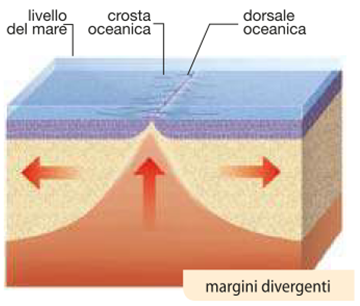
\includegraphics[width=.4\textwidth]{resources/margini-divergenti.png}
    \end{wrapfigure}

    Sono aree in cui si crea nuova litosfera oceanica. Coincidono con le dorsali oceaniche,
    ma includono anche i rift continentali, come la regione delle grandi fosse tettoniche
    africane. Le due placche ai lati della dorsale si accrescono, poiché si forma un nuovo
    fondale oceanico. La litosfera prodotta viene spinta lateralmente, con un moto
    divergente rispetto alla dorsale. Sono caratterizzati da un'intensa
    attività vulcanica e da una debole attività sismica.
    \wrapfill
    \vspace{-1cm}
    \begin{itemize}
        \item La litosfera si inarca e si frattura, permettendo la risalita del magma
            dall'astenosfera, che solidifica formando nuova crosta oceanica. La lava basaltica
            fuoriesce, raffreddandosi e ostruendo la frattura, che viene riaperta dalla tensione
            delle correnti del mantello;
        \item Le dorsali oceaniche espandono il fondale marino a velocità variabili, formando
            nuova crosta che si allontana dalla dorsale. Questo processo crea oceani in diverse
            fasi evolutive, dal rift embrionali come la Rift Valley africana agli oceani maturi
            come l'Atlantico.
    \end{itemize}
\end{snippet}

\subsection{Margini convergenti}

\begin{snippetdefinition}{margine-convergente}{Margine convergente}
    I \textit{margini convergenti} o \textit{margini di subduzione} (collisione) sono distruttivi e
    avvengono quando due margini si scontrano.
\end{snippetdefinition}

\begin{snippet}{margini-convergenti-expl}
    \setlength{\intextsep}{0pt}%
    \begin{wrapfigure}{l}{.55\textwidth}
        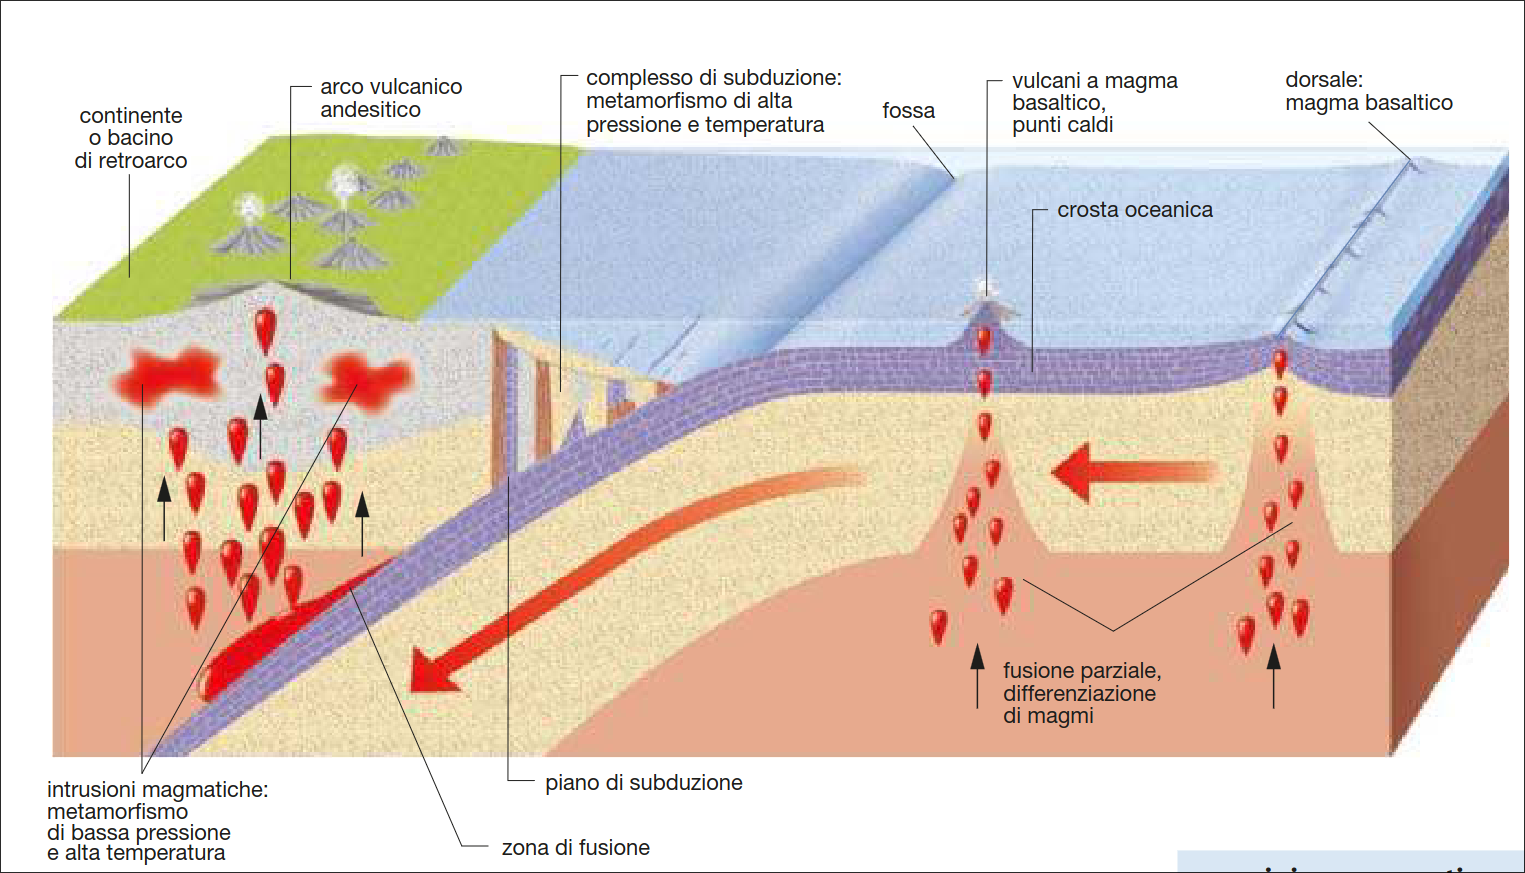
\includegraphics[width=.55\textwidth]{resources/margini-convergenti.png}
    \end{wrapfigure}

    Lungo questi margini, le placche contigue sono sospinte l'una contro l'altra.
    Coincidono con le catene montuose recenti e sono caratterizzati da fenomeni sismici
    molto violenti e da un'intensa attività magmatica, sia effusiva sia intrusiva.

    Il materiale che fonde, risale dando origine ad attività vulcaniche.
    Se i margini sono oceanica-oceanica, abbiamo una formazione di isole vulcaniche,
    altrimenti si tratta di margini oceanica-continentale.

    L'orogenesi avviene ai margini convergenti delle placche tettoniche, dove la collisione tra
    placche causa piegamenti e sovrascorrimenti che formano le montagne. Questo processo include la
    subduzione e la collisione continentale, creando catene montuose come l'Himalaya e le Alpi.
    \wrapfill

    \begin{itemize}
        \item I margini convergenti sono i confini tra placche tettoniche dove avviene la collisione.
            Esistono quattro tipi di convergenza:
            \begin{enumerate}
                \item Litosfera continentale vs. oceanica: la placca oceanica subduce sotto quella
                    continentale, formando una fossa oceanica e un arco vulcanico, con intensa
                    attività sismica (es. Ande);
                \item Litosfera oceanica vs. oceanica: una placca subduce sotto l'altra, formando
                    una fossa oceanica e un arco vulcanico insulare (es. Giappone, Filippine);
                \item Litosfera continentale vs. continentale: nessuna placca subduce, si formano
                    catene montuose tramite piegamenti e sovrascorrimenti (es. Himalaya, Alpi);
                \item Placca mista vs. oceanica: la litosfera oceanica subduce, mentre quella
                    continentale causa terremoti e deformazioni (es. margine tra placca
                    euroasiatica e africana).
            \end{enumerate}
    \end{itemize}
\end{snippet}

\subsection{Margini trasformi}

\begin{snippetdefinition}{margine-trasforme}{Margine trasforme}
    I \textit{margini trasformi} o \textit{margini conservativi} e di \textit{scorrimento},
    avvengono quando le placche si muovono in senso opposto a velocità differenti.
\end{snippetdefinition}

\begin{snippet}{margini-trasformi-expl}
    \setlength{\intextsep}{0pt}%
    \begin{wrapfigure}{l}{.45\textwidth}
        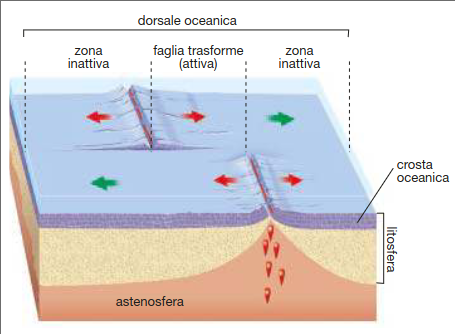
\includegraphics[width=.45\textwidth]{resources/margini-trasformi.png}
    \end{wrapfigure}

    Lungo questi margini, le placche scivolano l'una accanto all'altra, muovendosi in
    direzioni opposte o a velocità differenti. Coincidono con faglie trasformi e sono
    caratterizzati da una forte attività sismica, ma generalmente privi di attività
    vulcanica o magmatica.
    I margini trasformi non provocano vulcanismo ma violenti terremoti.
    \wrapfill
    \vspace{-1cm}
    \begin{itemize}
        \item I margini conservativi sono caratterizzati dallo scorrimento orizzontale delle placche
            tettoniche senza creare o distruggere litosfera. Le placche si muovono lateralmente
            lungo faglie trasformi, causando terremoti violenti ma senza formazione di montagne o
            vulcani significativi (es. Faglia di San Andreas);
        \item Le faglie trasformi nelle dorsali oceaniche interrompono la continuità delle dorsali,
            con movimenti opposti dei blocchi rocciosi, generando terremoti dovuti alla diversa
            velocità di espansione.
    \end{itemize}
\end{snippet}

\end{document}